\section{Square}
\label{sec:square}
If the source node $S$ is the center of a square that contains only default moves we can use these default moves as optimal moves. In doing so we can avoid to store these moves in the CPD and replace them with wildcards.\\ 
Let's take the toy map in Figure \ref{fig:toy_map} as example.\\
\begin{figure}[h]
	\centering
	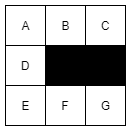
\includegraphics[width=0.3\columnwidth]{toy_map.png}
	\caption{A toy gridmap used as an example.}
	\label{fig:toy_map}
\end{figure}

For each node we build the maximum square centered in that node that contains only default moves and store the length of the side of this square. In Figure \ref{fig:example} we show the squares for node $A$ (\ref{fig:example_1}) and node $D$ (\ref{fig:example_2}); we can notice that squares can contain obstacles and exceed the dimension of the map as long as all the available moves inside of them are default moves. 

\begin{figure}[h]
      \centering
      \begin{subfigure}{.35\columnwidth}
      \centering
      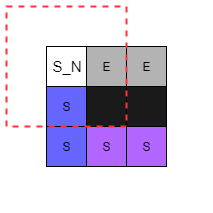
\includegraphics[width=.6\columnwidth]{square_nodeA.png}
        \caption{}
        \label{fig:example_1}
      \end{subfigure}%
      \begin{subfigure}{.35\columnwidth}
      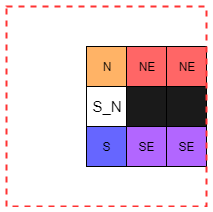
\includegraphics[width=.6\columnwidth]{./square_nodeD.png}
      \centering
        \caption{}
        \label{fig:example_2}
      \end{subfigure}
      \caption{\small Examples of squares computed for nodes $A$ and $D$}
      \label{fig:example}
    \end{figure}

While computing the CPD using the length of the sides we stored for each source node $S$ we can decide if a target node $T$ belongs to $S$'s square using the function $is\_in\_square$ (Algorithm \ref{alg:1}). If $T$ belongs to the square we store a wildcard instead of its move.\\
In Figure \ref{fig:results} we show the first move matrix and the array containing the length of the square side for each node.

\begin{figure}[h]
      \centering
      \begin{subfigure}{.35\columnwidth}
      \centering
      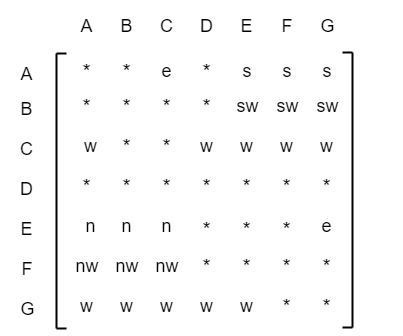
\includegraphics[width=.9\columnwidth]{cpd_square.png}
        \caption{}
        \label{fig:results_1}
      \end{subfigure}%
      \begin{subfigure}{.35\columnwidth}
      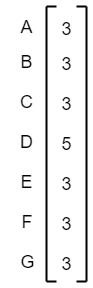
\includegraphics[width=.25\columnwidth]{sides_array.png}
      \centering
        \caption{}
        \label{fig:results_2}
      \end{subfigure}
      \caption{\small First move matrix and sides array for toy map}
      \label{fig:results}
    \end{figure}


\pjs{Why not store the distance, e.g. $side = 1$ instead of $side = 3$.
  It seems currently $side = 3$ and $side = 4$ give the same result!}


\begin{algorithm}
\KwIn{$S$, $T$, $side$}
\KwOut{$true$, $false$}
$\delta x$ $\gets$ $|S.x - T.x|$\\
$\delta y$ $\gets$ $|S.y - T.y|$\\
\eIf{$\delta x \leq (side-1)/2$ $\&$ $\delta y \leq (side-1)/2$}{\Return $true$}{\Return $false$}
\caption{is\_in\_square}\label{alg:1}
\end{algorithm}

 

\begin{algorithm}
\KwIn{$S$, $T$}
\KwOut{$move$}
$move$ $\gets$ \textsf{default}($S$,$T$) \\
$side$ $\gets$ \textsf{square}($S$,$T$) \\
$\delta x$ $\gets$ $|S.x - T.x|$\\
$\delta y$ $\gets$ $|S.y - T.y|$\\
\If{$\delta x \leq (side-1)/2$ $\wedge$ $\delta y \leq (side-1)/2$ $\vee$
    \textsf{CPD}($S$,$T$) = $\heur$}{\Return $move$}
\Return \textsf{CPD}($S$,$T$) 
\caption{Get next move algorithm for CPDs with squares and heuristic moves.}
\label{alg:2}
\end{algorithm}




